\section{ERTMS Level 2}

 %% The European Rail Traffic Management System (ERTMS) consists of
 %% several sub-systems. With regards to control and safety, these
 %% systems are typically designed to ensure safe operation of a
 %% particular area of railway known as a scheme plan. The ERTMS standard
 %% also outlines mechanisms allowing trains to pass between such regions
 %% (so-called handover protocols). In our work, we concentrate on safety
 %% within one region, and leave the handover mechanism for future work.

ERTMS Level 2 extends classical railway signalling. To this end its
location specific design\footnote{We focus here on one ERTMS/ETCS
  system controlling a single, geographic region.} extends the
classical notion of a scheme plan by information used for the radio
block centre (RBC). ERTMS safety analysis also requires train
characteristics such as maximum speed, acceleration and braking
curves.

\subsection{Scheme Plans}

A scheme plan is a well-established concept within the railway
domain. Figure~\ref{fig:station} depicts such a \emph{scheme plan} for
a pass-through station. It comprises of a track plan, a control table,
release tables and RBC tables. The \emph{track plan} provides the
topological information for the station. It consists of 8 tracks
(e.g.,\ BC) each with a length, 3 marker boards (e.g.,\ MB1), and two
points (e.g.,\ P2). A topological \emph{route} is a piece of railway
on which a train can travel, (typically) between two marker boards
(e.g., from MB1 to MB2). The {\em control table} describes under which
conditions a \emph{route} can be set.\footnote{It is a design
  decision whether a topological route appears in the control table. The
  routes in the table are those available for use by trains.}  For
example, a train can only proceed on route 1A when point P1 is in
normal (straight) position and tracks AA, AB and AC are clear, i.e.,
currently not occupied by any train. The \emph{release table} is used
to implement sequential release, a technique to improve
capacity. The release table describes when a point is again free to move
after being locked for a particular route. For example, when sending a
train on route 1A, point P1 is free to move already, when this train
has reached track AC. This allows to send another train on route 1B
before the first train has reached track AD and thus completely left
route 1A. Finally, the \emph{RBC tables} are used for %movement
calculations within the RBC.

\begin{figure}[H]
  \centering
 
\begin{tikzpicture}[scale=0.68,transform shape]
\fontfamily{Heletvica Narrow}{\fontsize{11}{11}\selectfont
\draw [->] (0,-0.8) to (1,-0.8);

\RWConnector{a0}{(0,-2)}
\RWConnector{a1}{(3,-2)}
\RWLinearUnitBelow{a0}{a1}{Entry}
\RWSignal{MB1}{(3,-2)}{MB1}
\RWConnector{a2}{(5,-2)}
\RWLinearUnitBelow{a1}{a2}{AA(1500m)}
\RWPoint{p101}{a3}{a4}{p101}{(6,-2)}
\RWLabelPointAboveLeft{a4}{a4}{P1}
\RWLabelLinearUnitBelow{a3}{a4}{AB(250m)}

\RWConnector{b5}{(9,-0.5)}
\RWLinearUnitBelow{p101}{b5}{BC(1500m)}
\RWConnector{b6}{(11,-0.5)}
\RWLinearUnitBelow{b5}{b6}{BD(1500m)}

\RWSignal{MB2}{(9,-0.5)}{MB2}
\RWConnector{a5}{(9,-2)}
\RWLinearUnitBelow{a4}{a5}{AC(1500m)}
\RWSignal{MB3}{(9,-2)}{MB3}
\RWConnector{a6}{(11,-2)}
\RWLinearUnitBelow{a5}{a6}{AD(1500m)}

\RWPointReverse{p102}{a7}{a8}{p101}{(12,-2)}
\RWLabelPointAboveRight{a8}{a8}{P2}
\RWLabelLinearUnitBelow{a7}{a8}{AE(250m)}

%\RWSignal{MB4}{(15,-2)}{MB1}
\RWConnector{a9}{(15,-2)}
\RWLinearUnitBelow{a7}{a9}{AF(1500m)}
\RWConnector{a10}{(17,-2)}
\RWLinearUnitBelow{a9}{a10}{Exit}
}
\end{tikzpicture}
\vspace{0.5cm}

\begin{tiny}
  \begin{tabular}{lll}
  Interlocking Tables: &
\begin{tabular}{|c|c|c|c|}
\hline
Route & Clear Tracks & Normal & Reverse \\
\hline \hline
1A & AA, AB, AC & P1 & \\
1B & AA, AB, BC & & P1 \\
2  & BD, AE, AF & & P2 \\  
3  & AD, AE, AF & P2 & \\
\hline
\end{tabular}
&
\begin{tabular}{|c|c|c|}
\hline
Point & Route & Release \\
\hline \hline
P1 & 1A & AC \\
P1 & 1B & BC \\
P2 & 2 & AF \\
P2 & 3 & AF \\
\hline
\end{tabular}\\ \quad \\
RBC Tables: &
\begin{tabular}{|c|c|}
\hline
Current Position & Continuation Routes \\
\hline \hline
Before MB1 & 1A, 1B \\
Before MB2 & 2 \\
Before MB3 & 3 \\
\hline
\end{tabular}
&
\begin{tabular}{|c|c|}
\hline
Granted Route & EOA \\
\hline \hline
1A & 3249m \\
1B & 3249m \\
2 & 6499m \\
3 & 6499m \\
\hline
\end{tabular}
\end{tabular}
\end{tiny}
\caption{Scheme Plan for a pass-through station.}
\label{fig:station}\label{fig:rbctables}
\end{figure}

We consider open scheme plans with entry and exit tracks
only. Furthermore, we assume that marker boards are placed at the end
of tracks, and that the speed limit is the same for all tracks.

\subsection{ERTMS System Architecture}

Once a scheme plan has been designed, a number of control systems are
implemented based around it. In the following we %systematically
identify the entities of ERTMS, describe their abstract behaviour and
determine the abstract information flow between them in line with the
design by Siemens Rail UK, see Figure~\ref{fig:arch}.

The \emph{controller} (manual or computerised) is responsible for
controlling the flow of trains through the railway network. The
controller completes this task by sending ``route request'' messages
to the interlocking. These route requests are dependent upon elements
such as the current timetable to be adhered to and details on
congestion within the network. For simplicity, we abstract from
``route cancel'' and ``acknowledgement'' messages.

The \emph{interlocking} is responsible for setting and granting
requested routes. Once the controller has requested a route, the
interlocking will use information on current track occupation and
point settings (from the track equipment) to determine if it is safe
for the requested route to be set. Whether a route can be set or not
is computed in a process based upon the conditions stipulated by the
control table, see Figure~\ref{fig:station}. Once the interlocking has
checked that all points on the route are free to move or already in
the right position, it will send a ``route available'' message to the
RBC (Radio Block Centre). This informs the RBC that the route is free
for use, however it is not yet reserved for a train. The RBC initiates
the process of locking a route for a particular train by sending a
``request to proceed'' message to the interlocking. On receiving this
message, the interlocking will then ensure that, based on the control
table, all tracks for the route are free and that the points are
indeed locked in the required positions. Once this step is completed,
the interlocking sends a ``proceed'' message to the RBC indicating
that a train can use the route.

The \emph{RBC}'s main responsibility is to take the route information
presented by the interlocking and use it to manage the movement of
trains across geographic positions on the railway. To do this, the RBC
and trains use the notion of a \emph{movement authority}. A movement
authority is an area of geographical railway that a train is permitted
to move within. The furthest point along the railway to which a train
is permitted to move is indicated by a point known as the \emph{end of
  authority} (EoA) which is given to a train by the RBC. As a train
moves across the railway network, it uses beacons on the track to
continually calculate its position. When it is nearing its EoA, it
makes a new ``movement authority request'' to the RBC indicating that
it would like its movement authority to be extended. After receiving
this request, the RBC will map the physical location of the train to
an available continuation route that has been presented to it by the
interlocking.\footnote{At this point, there should be maximally one
  route available that matches a particular train. This is ensured by
  the requests from the controller and also the ability of the
  interlocking to deny requests for conflicting routes} This
calculation is performed based on a look-up table designed as part of
the RBC for a scheme plan, an example of such a table is provided in
Figure~\ref{fig:rbctables}. It will then issue a ``request to
proceed'' message to the interlocking for this route. Once the RBC has
received a ``proceed'' message from the interlocking, it will compute,
based on the route that has been granted, a new EoA for the
train. Again, this information is provided by a look-up table, see
Figure~\ref{fig:rbctables}. This new EoA is then finally sent as a
``movement authority'' message to the train.

With regards to \emph{trains}, their behaviour is parameterised by
maximum speed, acceleration and braking curves. We make a maximum
progress assumption for trains, i.e., trains are running as fast and
as far as possible. Namely, if a train has a movement authority beyond
its current position it will accelerate towards its maximum
speed. When the maximum speed is reached, the train will continue to
travel at this speed. Whilst accelerating or travelling at maximum
speed the train will start braking at the last possible time in order
not to overrun its EoA. Trains are guided by the track layout,
respecting the positions to which the interlocking has set points. As
trains move along the track, track equipment senses track occupation
and reports it to the interlocking.
%
%% \begin{figure}[h]
%% \centering
%% \begin{tiny}
%% \begin{tabular}{|c|c|}
%% \hline
%% Current Position & Possible Continuation Routes \\
%% \hline \hline
%% Before MB1 & 1A, 1B \\
%% Before MB2 & 2 \\
%% Before MB3 & 3 \\
%% \hline
%% \end{tabular}
%% \quad
%% \begin{tabular}{|c|c|}
%% \hline
%% Granted Route & EOA \\
%% \hline \hline
%% 1A & 3249m \\
%% 1B & 3249m \\
%% 2 & 6499m \\
%% 3 & 6499m \\
%% \hline
%% \end{tabular}
%% \end{tiny}
%% \caption{RBC tables for calculating continuation routes and end of authorities.}
%% \label{fig:rbctables}
%% \end{figure}
%
We assume that \emph{track equipment} (points, track circuits, beacons
etc.) functions correctly and that points move instantaneously. This
is justified as our verification aim is to establish correctness of
the location and train specific design parameters for a ERTMS system
for a single geographic region. Therefore, we refrain from modelling
track equipment.

\begin{figure}[H]
\centering
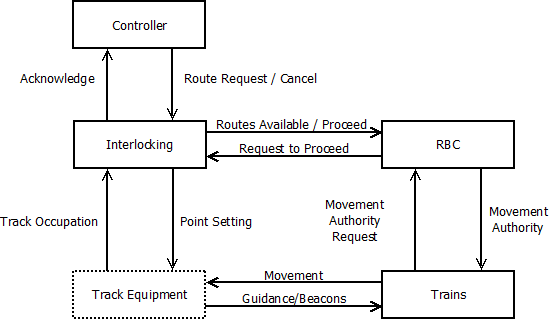
\includegraphics[scale=0.45]{images/Architecture.png}
\caption{ERTMS control architecture.}
\label{fig:arch}
\end{figure}

\subsection{Safety Conditions}
\label{sec:safetycond}
In the context of ERTMS, several high level safety conditions have
been discussed such as collision freedom or derailment on a point.  In
this paper, we focus on collision freedom, i.e., excluding the
possibility that two trains collide.  In the context of classical
signalling systems, this property usually is formulated logically,
e.g., we verify that there are never two trains on the same track
\cite{sttt14}. In contrast, for ERTMS we rather consider the physical
invariant: the distance between trains never falls below a
minimum threshold.

%% MR: excellent text - but we should use it in the introduction of 
%% the error-injection section
%%
%% As we illustrate later in Section\ref{sec:errorInjection}, there are a
%% number of ways in which this condition can be violated within
%% ERTMS. In this work, we assume that the generic dynamic behaviour of
%% the interlocking, RBC and any trains is correct and that the mistakes
%% we are looking for are within the parameters to these models. For
%% example, mistakes in the design of the control and release tables for
%% an interlocking can lead to a violation of this property. Similarly,
%% mistakes in the design of mappings between routes and end of
%% authorities for use within the RBC can also violate this
%% property. Finally, if a train has incorrect parameters input for
%% computing braking distances, the the property may once again be
%% violated.

